\documentclass[nolineno]{ieeeaccess}
\usepackage{cite}
\usepackage{amsmath,amssymb}
\usepackage{graphicx}
\usepackage{booktabs}
\usepackage{url}
\usepackage[hidelinks,bookmarks=false]{hyperref}
% Correct intentional zero-width containers in the supplied class without
% changing page geometry, fonts, colors, content placement, or class-file bytes.
\usepackage{etoolbox}
\makeatletter
\patchcmd{\@maketitle}{\noindent\box99}{\noindent\makebox[\titlewidth][l]{\box99}}{}{\PackageError{journal}{Abstract container patch failed}{}}
\patchcmd{\@maketitle}{\noindent\box88}{\noindent\makebox[\titlewidth][l]{\box88}}{}{\PackageError{journal}{Keywords container patch failed}{}}
\def\journal@oddfoot#1{\raisebox{#1}{\hbox to\textwidth{%
{\footervolfont VOLUME\ \thevol, \theyear}\hfill{\footerpagefont\thepage}}}}
\def\journal@evenfoot#1{\raisebox{#1}{\hbox to\textwidth{%
{\footerpagefont\thepage}\hfill{\footervolfont VOLUME\ \thevol, \theyear}}}}
\let\journal@headings\ps@headings
\def\ps@headings{\journal@headings\def\@oddfoot{\journal@oddfoot{8pt}}\def\@evenfoot{\journal@evenfoot{8pt}}}
\let\journal@titlepage\ps@titlepage
\def\ps@titlepage{\journal@titlepage\def\@oddfoot{\journal@oddfoot{3pt}}\def\@evenfoot{\journal@evenfoot{3pt}}}
\ps@headings
\makeatother

\graphicspath{{figures/}{template/assets/}{./}}
\begin{document}
\history{Draft prepared for author review.}
\doi{Not assigned; draft manuscript}
\vol{--}\year{2026}
\title{Smart Safety Tag: Design and Verification of a Wearable-Assisted Personal Safety System}
\author{\uppercase{Bala Rakesh Gundapaneni}, \uppercase{Abdul Basith Syed}, \uppercase{Jagadeeshbabu Borru}, and \uppercase{Naga Sravanthi Puppala}}
\address{Affiliations and corresponding author details to be confirmed.}
\markboth{Smart Safety Tag}{Smart Safety Tag}
\begin{abstract}
Smart Safety Tag is a prototype for sharing an emergency alert with trusted contacts. The project combines an Android-first application, an application programming interface, an administrative portal and designs for a custom wearable PCB and charging adapter. The app supports a confirmed SOS action and guardian management; the backend stores emergency events and provides best-effort notifications. The tag design includes an ESP32-S3 module, a button, motion and audio peripherals, local feedback and a protected charging path. This article describes the design and distinguishes software checks and engineering calculations from physical measurements. The available checks include 24 passing mobile unit tests, 57 passing backend tests using in-memory repositories and a successful administrative type check. Saved design reports record no PCB design-rule violations, and the hardware-test firmware has been compiled. No assembled tag was available for physical validation, and the wearable emergency connection and keyword inference remain unimplemented. The work therefore documents a design and its current evidence; it does not establish improved emergency response or the performance of a complete wearable system.
\end{abstract}
\begin{keywords}Personal safety, wearable devices, emergency notification, Bluetooth Low Energy, mobile applications, prototype verification.\end{keywords}
\maketitle
\raggedbottom
\section{Introduction}
An alert is only the beginning of a response: someone must receive it, understand what happened and decide how to help. A wearable button could make the initial action easier, while a companion phone could provide location and network access. In practice, each step depends on power, permissions, connectivity and the availability of trusted contacts. A working interface or a completed PCB layout cannot, on its own, show that help will reach the person who needs it.

The Smart Safety Tag repository brings together an Android-first app, a FastAPI backend, an administrative web portal and a separate wearable design. The software can create an emergency from the app. The hardware has reached a different stage: its board layout and peripheral-test firmware are available, but the records contain no measurements from an assembled tag. The test firmware does not send an SOS event from the wearable to the phone.

The paper describes how these pieces are intended to fit together, explains which software and hardware functions are present, and traces the available checks to the claims they can support. It also sets out the work needed to evaluate the complete path from a wearable action to a guardian response. We report no user study, comparative performance experiment or physical safety qualification.

\section{Related Work}
Personal-safety applications and wearable alerts have been explored in earlier work. One IEEE conference paper describes a device with its own GPS, cellular messaging and camera~\cite{wearable2025}. A published patent application describes a wearable alert button that communicates with a smartphone and contacts~\cite{patent2024}. Such work establishes that the general combination of a button, phone, Bluetooth and notifications is not new. Our discussion concerns this project's implementation and evidence, not a patentability or freedom-to-operate opinion.


\subsection{Design Choices in Prior Systems}
The division of work between a wearable and a phone varies across designs. The device described by Purnima \textit{et al.} includes on-board GPS, cellular messaging and a camera~\cite{wearable2025}; its direct communication path has different hardware and service dependencies from a phone-assisted system. Wankhede \textit{et al.} describe a bracelet linked to an app over BLE, with location and feedback components~\cite{wankhede2025}. A phone-connected alert also appears in~\cite{patent2024}. These publications inform the design comparison but were not used as experimental baselines.

In the proposed Smart Safety Tag architecture, the phone supplies location and Internet access. That choice leaves cellular and GPS subsystems off the tag, but it also makes the phone, its connection and the app's operating state part of the alert path. Because the wearable emergency link has not been implemented in the test firmware, this choice does not support a comparison of response time, cost, range or reliability. The contribution here is a documented design at a defined stage of development.

Location and alert data can also reveal a person's routines. Barman \textit{et al.} found that patterns in encrypted Bluetooth traffic from tested wearables could disclose information about device use~\cite{barman2021}. Their work does not demonstrate an attack on this project, but it makes traffic metadata a useful subject for a future review of the planned BLE link. On the phone, access to location also depends on permission and operating-system behavior when an app moves between foreground and background states~\cite{androidlocation}.


\subsection{Safety and Security Literature}
Prior research spans manually activated alerts, sensor-based inference and several communication paths. Farooq \textit{et al.} review sensors and communication choices used in wearable safety research~\cite{farooq2023}. Roy \textit{et al.} describe a device that combines physiological monitoring with alerts to a guardian application~\cite{roy2024}; Sonia \textit{et al.} discuss a separate sensor-based protection system with remote communication~\cite{sonia2024}. Their approaches and evaluations differ, so their reported outcomes cannot be assumed for Smart Safety Tag.

Other designs consider automatic recognition as an alert trigger. Hariprasad \textit{et al.} describe an architecture using edge inference and additional communication technologies~\cite{hariprasad2025}. The Smart Safety Tag board design includes a microphone and accelerometer, but the current test application has neither a trained distress-keyword model nor an automatic fall detector. Having a sensor on a schematic is not the same as having an evaluated detector. Research on personal-safety apps also examines how people choose responses in threatening situations, a question that technical tests alone cannot answer~\cite{just2019}.

The proposed wearable link also needs a security design. Kurt Peker \textit{et al.} examined BLE security features in selected consumer devices~\cite{peker2022}, while Givehchian \textit{et al.} evaluated physical-layer tracking attacks against mobile devices~\cite{givehchian2022}. These studies concern the devices they tested, not the unassembled tag. Together with the Bluetooth traffic-analysis study~\cite{barman2021}, they motivate explicit evaluation of pairing, authentication and privacy once the emergency link exists.

\section{System Architecture}
\begin{figure*}[t]
\centering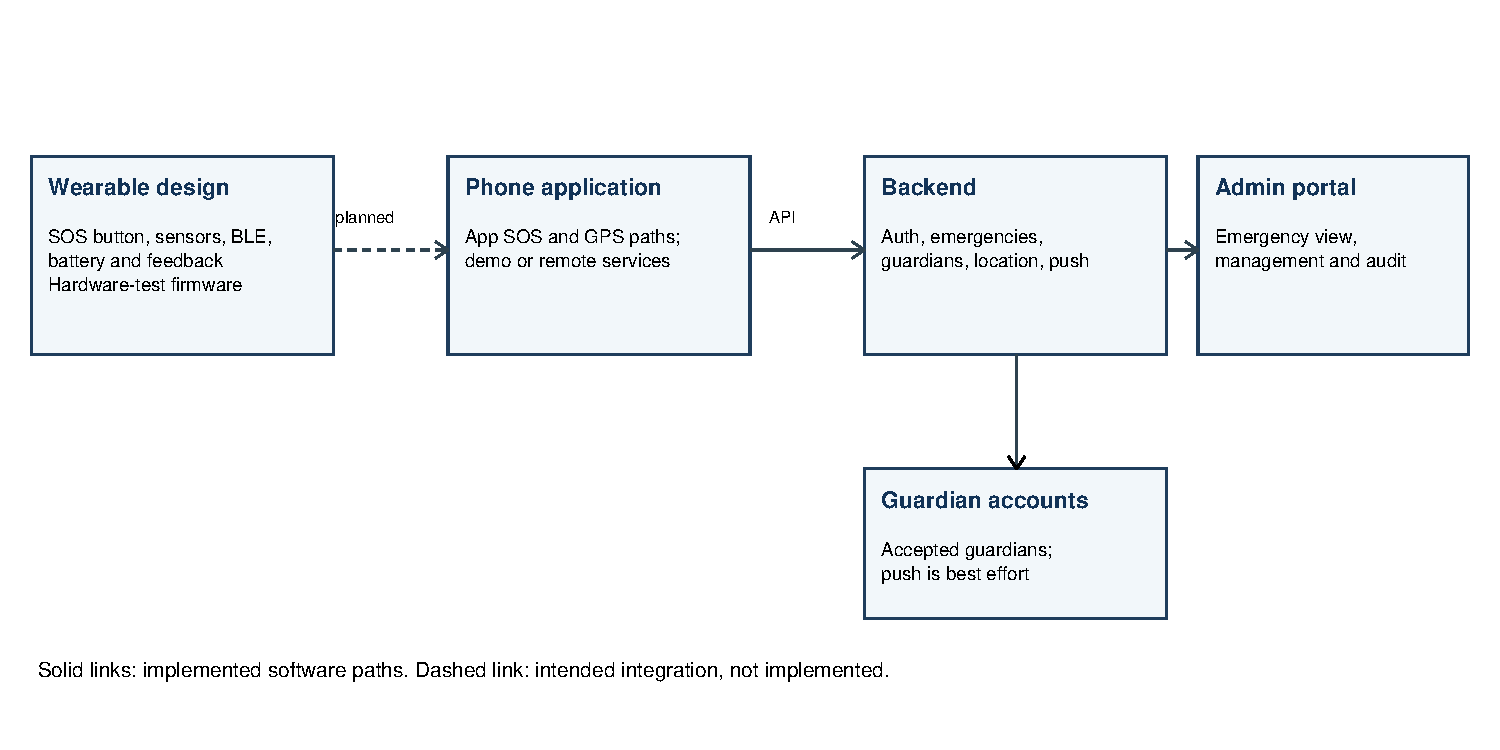
\includegraphics[width=\textwidth]{architecture.pdf}
\caption{System overview. Solid lines show software paths in the repository; the dashed wearable-to-phone connection remains planned. The diagram does not establish availability or delivery.}
\label{fig:architecture}
\end{figure*}
Figure~\ref{fig:architecture} separates the existing software paths from the intended wearable connection. The app contains onboarding, sign-in, home, tracking, guardian and profile screens. When the backend is configured and a user is signed in, remote services handle the relevant data; otherwise the interface can use local demonstrations. A demo alert does not establish that a message left the phone. Native location helpers and background-task code are present, but their behavior on a device depends on permissions, configuration and operating-system conditions.

The backend offers authenticated routes for accounts, devices, guardians, locations and emergencies. It hashes passwords with Argon2 and uses short-lived access tokens with rotating refresh tokens. Guardian access depends on an accepted invitation. With a real database pool, the emergency record and its initial event are written in one transaction. The admin portal uses role-checked routes for monitoring and management. WebSocket events and push notifications are best-effort mechanisms; neither alone proves that a recipient has acknowledged an alert.

\subsection{In-App Emergency Path}
An app-originated SOS requires user confirmation. In remote mode, the client attempts to attach a phone location and sends an application-button trigger to the server. If the location attempt returns no fix, the request can proceed without coordinates. Missing or delayed location may leave a guardian with less useful context, and the current code establishes no guaranteed delivery time. With a suitable provider and valid tokens, the backend can attempt push delivery to the owner and accepted guardians. The mock notification provider records a log rather than delivering a message.

The emergency lifecycle has active, acknowledged, resolved and cancelled states. The service checks the permitted transitions and records events as the status changes. An authenticated channel supplies emergency updates to the administrative portal. Connectivity, mobile process restrictions, notification failures and the guardian's availability can all interrupt the wider response even when an individual software operation succeeds.


\begin{figure*}[t]
\centering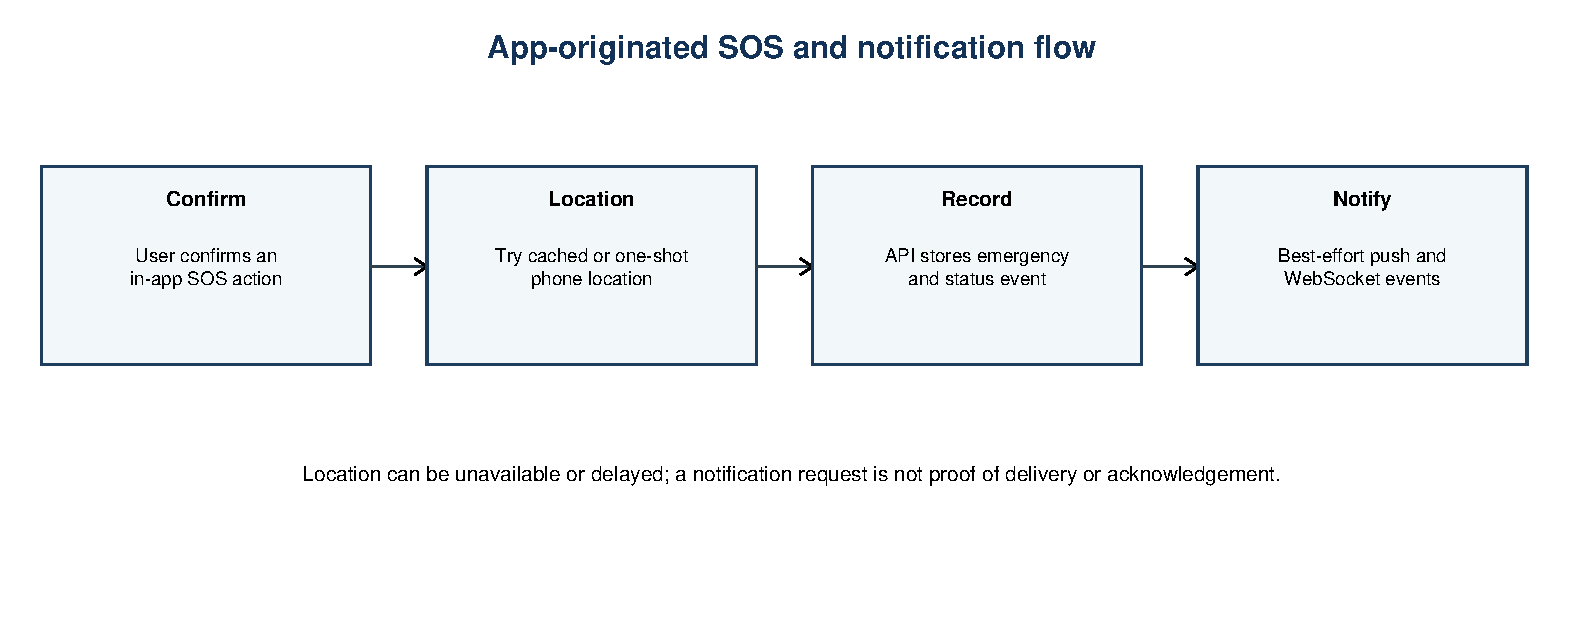
\includegraphics[width=\textwidth]{sos_flow.pdf}
\caption{App-originated SOS workflow. Push notifications and real-time events are best effort; the wearable emergency link is not implemented.}
\label{fig:sos-flow}
\end{figure*}
\subsection{Mobile Client and Service Selection}
The interface groups onboarding, authentication, home, tracking, guardians and profile functions into separate screens. A service layer supplies data to those screens. Its selector uses remote data services for a configured, signed-in session and local mocks when a backend session is unavailable. Authentication has its own selection rule: when an API URL is configured, sign-in targets the remote service. This arrangement supports a demonstrable interface without implying that simulated alerts have been sent.

The local store retains onboarding completion, a minimal profile, guardians and preferences. In demonstration mode it can also display a location, device state and recent alert without a live backend or a physical tag. Those screens illustrate the interface, not measured radio connectivity or location accuracy. Remote device responses are mapped into presentation models; a device card is therefore a display of server-reported state, not proof of an active BLE connection.

\subsection{Location and Permissions}
Native location helpers request foreground and background permissions and register location updates. When a signed-in user has enabled sharing and the relevant preference, a foreground watcher can update the last-fix value and attempt an upload. A background task can also submit updates where the operating system and granted permissions allow it. The web path does not use these native modules. The intervals in the configuration are requested intervals, not measurements of the actual delivery frequency.

For a remote SOS, the client uses a cached fix if one exists; otherwise it tries a one-shot location request. A request can be submitted without coordinates if no fix is returned. The helper accepts a timeout argument but does not enforce it, so the implementation does not establish an upper bound on waiting time. It also imposes no documented maximum age on the cached fix. Device tests should cover denied permissions, stale fixes, background restrictions and reconnection. Android documents separate foreground and background permission behavior~\cite{androidlocation}, but the presence of permission-handling code does not establish success on every target device.

\subsection{Guardians, Status and Event Delivery}
A user can invite a guardian by email. The backend can link a pending invitation to a subsequently created account, and the invited guardian can accept or reject it. The owner and accepted guardians may read protected emergency and location records. An active emergency can move to acknowledged, resolved or cancelled; an acknowledged emergency can move to resolved or cancelled. Resolved and cancelled states are terminal. The service records accepted changes, but a status value does not itself prove that a person has taken action.

When a database pool is available, emergency creation writes the record and initial event in a transaction. Push delivery is dispatched as a background task where configured, while WebSocket emission is best effort. For push, the service selects the owner and accepted guardians and resolves their registered tokens. The mock provider logs instead of sending, and an incorrectly configured provider may fall back to mock mode. A provider request, arrival on a guardian's device and acknowledgement by that guardian are separate events; none has a measured delivery rate in the repository.

The administrative portal uses the same backend for emergency monitoring, user and device management, location history and audit information. The server checks roles on administrative routes. Handling these records also requires decisions about access, retention, logging and incident response. Those are operational requirements, not evidence that an independent security assessment has been completed. Figure~\ref{fig:sos-flow} shows the app-originated workflow; it does not show a completed physical-button connection.


\subsection{Records and Access Boundaries}
The database schema keeps guardian relationships, location fixes, emergencies and emergency events in separate tables. A guardian record belongs to a protected user and can be linked to a guardian account; its status records whether the invitation is pending, accepted, rejected or removed. The database prevents duplicate guardian email entries for the same protected user. An invitation by itself does not grant access: the service checks the accepted relationship when another user requests protected location or emergency data.

Location records contain latitude, longitude, a source, a recording time and, when supplied, an accuracy estimate and device reference. The schema constrains coordinate ranges and requires a positive accuracy value when one is provided. Location reads are authorized for the owner or an accepted guardian, and a submitted device identifier must belong to the submitting user. These rules describe the implemented data path; they do not establish that a phone's position is current or that its reported accuracy is correct. A missing location is different from a confirmed position, and consumers of an emergency record should be able to distinguish them.

An emergency has its own identifier, protected user, trigger type, status, timestamps and optional device, coordinates and note. The associated event table records status transitions and the actor where available. This separation allows the application to maintain a timeline without treating every location update as an emergency. The schema permits several trigger labels, but a permitted label is not evidence that a corresponding wearable detector has been implemented. Database constraints and service authorization are complementary: neither replaces the need to test the deployed database, operational configuration and client behavior.

\section{Wearable Design}
The wearable design centers on an ESP32-S3-MINI-1 module with BLE capability~\cite{esp32}. Its other components include an SOS button, LIS2DW12 accelerometer, PDM microphone, MAX17048 fuel gauge, RGB indicator, vibration motor and protected nominal 400 mAh cell. A separate adapter supplies power through contacts with an eFuse on the adapter side. In the intended architecture, GPS and Internet access come from the phone.

The specified tag board measures 60 by 42 mm; the charging adapter measures 32 by 22 mm. The power design uses a BQ25185 charging path~\cite{charger} and a TPS63802 regulator~\cite{regulator}, with a temperature-sensing circuit intended to inhibit charging outside a modeled window. Runtime values in the project power budget are calculations based on assumed currents. Charging behavior, antenna clearance in an enclosure, battery safety and mechanical fit remain to be measured.

The included ESP-IDF application exercises peripheral APIs, logs sensor readings, drives feedback, captures short audio windows and supports basic BLE advertising and connection handling. It stays awake and is a hardware-test program. It has no custom emergency BLE service, keyword inference, phone-notification workflow, fall detector or product sleep/wake implementation. The presence of a trigger type in a server schema does not mean that the corresponding physical detector exists.


\begin{figure*}[t]
\centering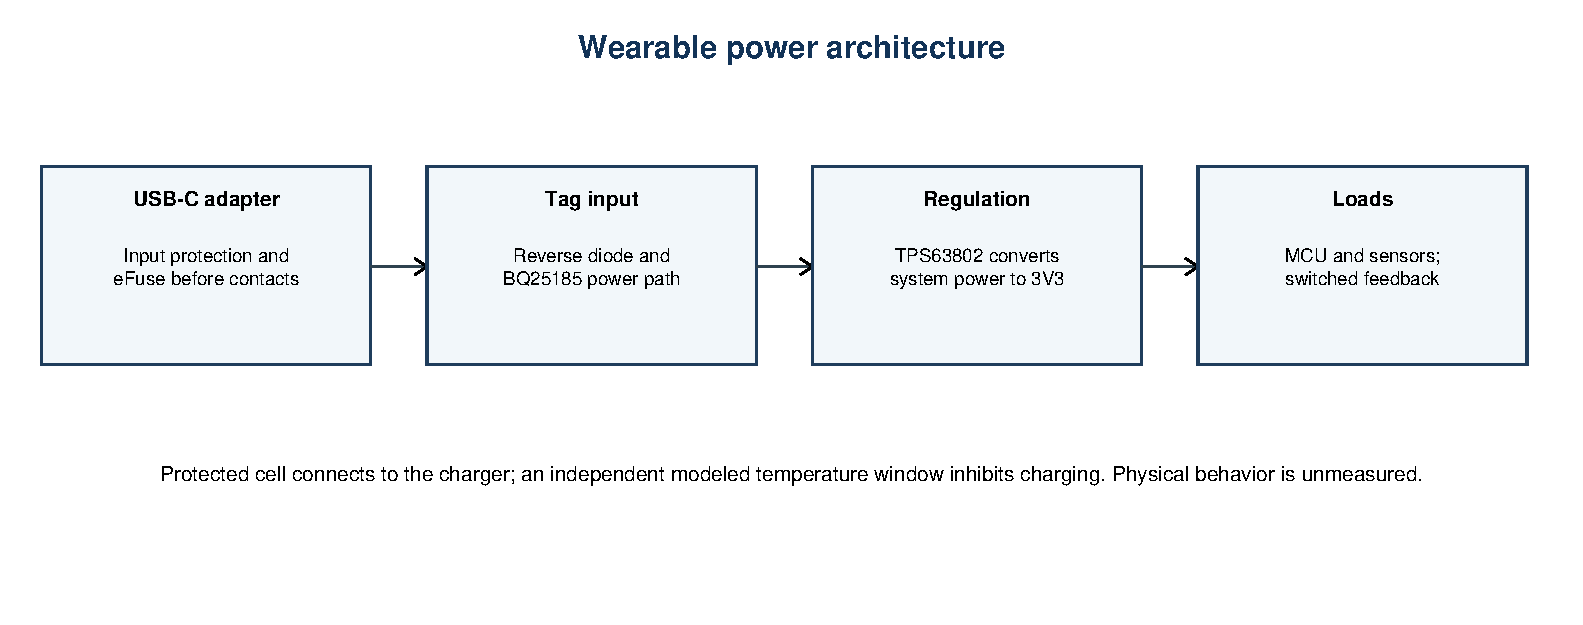
\includegraphics[width=\textwidth]{power_path.pdf}
\caption{Designed wearable power path. The cell, temperature interlock and adapter require physical charging and load tests.}
\label{fig:power-path}
\end{figure*}
\subsection{Sensing and Feedback}
The selected ESP32-S3 module combines processing and BLE with 4 MB flash and 2 MB PSRAM~\cite{esp32}. A LIS2DW12 accelerometer and MAX17048 battery gauge use I\textsuperscript{2}C; their alert or interrupt signals are routed to processor pins~\cite{lis2dw12,fuelgauge}. The button input is active low and includes a pull-up and filter. The hardware-test program polls it and logs transitions. These observations describe the design and source code: interrupt behavior, button response and gauge accuracy have not been measured on an assembled tag.

A switched 3.0 V supply supports PDM microphone capture. The test program records short mono windows and logs amplitude statistics; it does not run a keyword model. The RGB indicator and vibration motor provide local feedback in the test program. A motor pulse does not establish that a notification reached another person. The PCB also provides an acoustic opening and antenna keepout. Their effectiveness depends on the enclosure, battery, clip and nearby materials, so both acoustic and RF behavior need assessment in a fitted assembly.

\subsection{Charging and Power Design}
The path in Fig.~\ref{fig:power-path} begins at a USB-C adapter with an eFuse before the exposed contacts~\cite{efuse}. On the tag, a reverse-protection diode precedes the BQ25185 charger and system-power path~\cite{charger}; a TPS63802 supplies the nominal 3.3 V rail~\cite{regulator}. The protected cell connects to the charger, and the motor and microphone have switched supply paths. These choices address specific design concerns, but a schematic cannot establish behavior under contact shorts, reversed polarity, heating or component failure.

A thermistor and comparator window are intended to inhibit charging independently of the processor. The electrical model accounts for resistor and thermistor tolerances, charger bias, supply variation, comparator offset and hysteresis. Its modeled corners inhibit charging at 0 and 45 degrees Celsius and permit it at 25 degrees Celsius. These are modeled points rather than observed trip thresholds. Actual sensor-to-cell coupling, hysteresis, lag and open- or short-sensor faults remain to be tested.

The feedback divider uses 511 k\(\Omega\) and 91 k\(\Omega\) resistors with a nominal 0.5 V reference, giving an estimated output of 3.308 V. The power budget allocates 500 mA for a rail test and gives an example discharge-end battery current of approximately 0.77 A, assuming 85 percent conversion efficiency and a 120 mA motor load. These are design assumptions, not simultaneous current measurements. Startup, ripple, load transients and pack protection require tests with the fitted hardware.

\begin{table}[t]
\caption{Battery-side runtime estimates under assumed operating currents}
\label{tab:runtime}
\centering
\begin{tabular}{lrr}
\toprule
Assumed operating scenario & Current & Runtime \\
\midrule
BLE monitoring; microphone off & 8 mA & 40 h \\
Continuous audio processing & 80 mA & 4 h \\
Sustained emergency activity & 170 mA & 1.9 h \\
\bottomrule
\end{tabular}
\par\smallskip\footnotesize Calculated from an assumed 320 mAh usable capacity. The test firmware does not implement the proposed operating modes; no runtime is measured.
\end{table}

Table~\ref{tab:runtime} shows how strongly a runtime estimate depends on average current. The planning relation \(T=C_{\mathrm{usable}}/I_{\mathrm{avg}}\) gives 40 h for an assumed 320 mAh usable capacity and 8 mA average current. Capacity reserve, conversion losses and operating currents in the calculation are assumptions. Actual runtime will depend on the radio schedule, regulator, temperature, aging, motor starts and final firmware. The included test firmware remains awake and does not implement the table's proposed low-power modes.


\subsection{Custom PCB and Assembly Organization}
The fabrication package contains two custom boards: a wearable tag and a separate charging adapter. Both use two-layer FR-4 with a specified 1.0 mm finished thickness. The tag measures 60 by 42 mm and contains 83 footprints, including bare pads and connectors; the 32 by 22 mm adapter has 16. These are CAD counts, not evidence of manufactured boards. The tag schematic separates the processor, microphone, accelerometer, charging, regulation, battery monitoring, feedback and programming protection into functional sheets.

\begin{figure*}[t]
\centering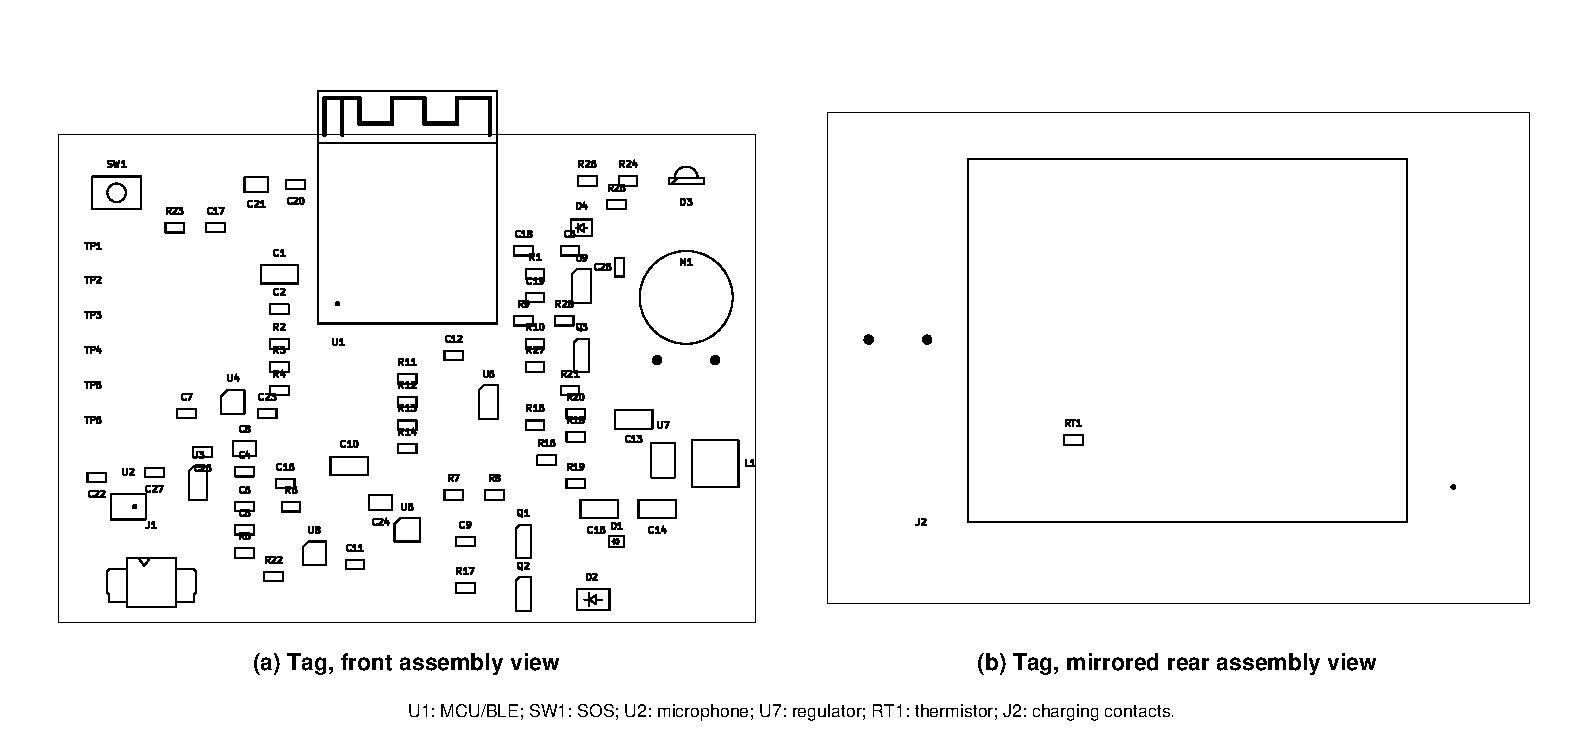
\includegraphics[width=\textwidth]{tag_board.pdf}
\caption{Tag PCB assembly views from the CAD exports. The rear view is mirrored and shows the intended battery envelope and thermistor position; no assembled tag is pictured.}
\label{fig:tag-board}
\end{figure*}
Figure~\ref{fig:tag-board} shows front and mirrored rear assembly views from the CAD exports. The processor module sits near the upper edge; its antenna extends 3.75 mm beyond the outline and has an all-layer keepout. A battery, clip, magnet or enclosure placed nearby could still change radio behavior. A representative RF test must therefore include the intended mechanical surroundings rather than testing an exposed board alone.

The rear CAD view marks the thermistor and battery envelope, but cannot show whether the cell is actually attached or thermally coupled. The manufacturing notes specify an insulating thermal interface and cell support. The two rear charging contacts have a specified 7.5 mm pitch. Because the rear view is mirrored, mating polarity should be checked against the electrical nets and board coordinates. Retention, spring-pin compression and contact wear remain mechanical tasks for a prototype.

\begin{figure*}[t]
\centering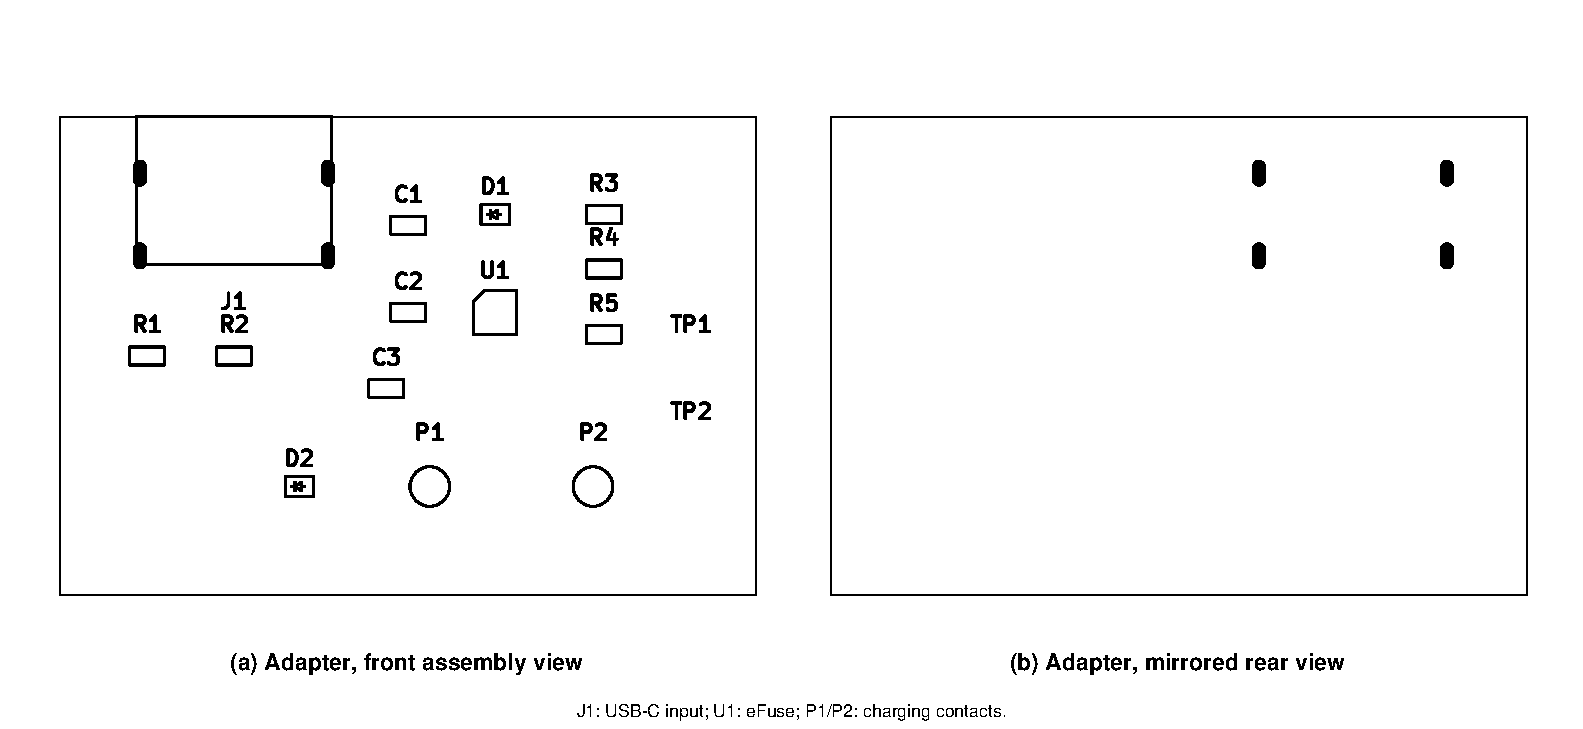
\includegraphics[width=\textwidth]{adapter_board.pdf}
\caption{Charging-adapter CAD views. The front view shows the USB connector and contacts; the rear view is mirrored. The design has not been physically tested.}
\label{fig:adapter-board}
\end{figure*}
The adapter in Fig.~\ref{fig:adapter-board} uses a power-only USB-C input and places an eFuse ahead of its spring-pin outputs. Its specified connector requires a board thickness of 1.0 \(\pm\) 0.10 mm. The adapter protection and the tag's reverse-blocking diode serve separate functions; neither has been qualified through a physical short-circuit or polarity-reversal test. The adapter supplies power and does not provide the USB data path for programming.

\subsection{Interface and Component Mapping}
Table~\ref{tab:components} maps the main subsystems to their interfaces and evidence. The accelerometer and fuel gauge share I\textsuperscript{2}C, while the microphone sends PDM data to the processor. Audio and motor supplies are switched independently in the circuit. Button, charger-status, fuel-alert and accelerometer-interrupt signals are assigned to processor pins. The interface definition also generates the firmware pin header, giving the design and test source a common mapping. The assignments still need to be checked against the fitted board.

\begin{table*}[t]
\caption{Main PCB subsystems and their current evidence}
\label{tab:components}
\centering
\begin{tabular}{p{0.18\textwidth}p{0.25\textwidth}p{0.23\textwidth}p{0.23\textwidth}}
\toprule
Subsystem & Design selection & Interface or role & Evidence boundary \\
\midrule
Processor and radio & ESP32-S3-MINI-1-N4R2 & MCU and BLE & Test firmware builds; RF operation unmeasured \\
Motion and battery & LIS2DW12; MAX17048 & I\textsuperscript{2}C and alert pins & Raw peripheral tests; calibration pending \\
Audio and feedback & IM67D128B, RGB LED, motor & PDM input; switched outputs & Short capture and pulse in test source only \\
Charging and supply & BQ25185; TPS63802; TLV7042 & Charging, regulation, thermal inhibit & Electrical model and CAD; physical checks pending \\
Adapter & USB-C input; TPS2595 eFuse; pogo pins & Protected power contacts & Fabrication design; contact behavior unmeasured \\
\bottomrule
\end{tabular}
\end{table*}

Six pads expose 3.3 V, ground, UART transmit and receive, boot control and enable. The documented procedure enters the bootloader manually; the charging adapter has no automatic serial boot control. GPIO26 is reserved for the selected module's PSRAM and remains unassigned. A block diagram alone cannot reveal every reserved-pin, voltage-domain or programming issue. The interface map and build record aid design review, but a boot log from a manufactured board is still needed.

The microphone uses a switched 3.0 V domain and a suitably limited clock signal~\cite{micdatasheet}. The test configuration captures 16 kHz mono PCM with a 2.048 MHz PDM clock. Its footprint has a 0.40 mm unplated acoustic hole that must remain clear during assembly and align with the enclosure. A completed DMA transfer or nonzero amplitude does not establish sensitivity, speech-recognition quality or emergency-detection performance.

\subsection{Layout, Fabrication and Protection Tradeoffs}
The fabrication specification calls for nominal 35 \(\mu\)m copper on both outer layers and an ENIG finish with exposed charging and test contacts. Minimum design clearances are 0.13 mm copper-to-copper and 0.15 mm copper-to-hole; the standard via has a 0.60 mm pad and 0.30 mm finished drill. Dense pads and the microphone footprint require narrow fanouts on the tag. A board house must confirm these requirements: they are not measurements from a manufactured lot. The package includes Gerber, drill and placement exports with manifests linking them to design sources.

The charging design selects a nominal 150 mA current for a protected 400 mAh battery. A board-mounted NTC thermistor and the TLV7042's open-drain comparator outputs form a window intended to inhibit charger enable outside the modeled range~\cite{comparator}. The processor has a separate inhibit path. Manufacturer guidance discusses NTC sensing for batteries~\cite{ntcapplication}; in this assembly, its usefulness depends on thermal coupling to the cell. CAD placement cannot establish that coupling, and the actual thresholds and open/short response remain unmeasured.

A capacitor's nominal value also differs from its effective value in a working circuit. The design record replaced an initial 10 \(\mu\)F input part with a 22 \(\mu\)F part after considering DC-bias derating. Applying the documented allowances of 50 percent bias loss, 20 percent negative tolerance and 15 percent temperature reduction gives \(22\times0.50\times0.80\times0.85=7.48\) \(\mu\)F. This arithmetic allowance is neither a guaranteed measured capacitance nor proof of converter stability. The fitted part and operating conditions still require checks for effective capacitance, aging, startup and load response.


\subsection{Button Input and Test Firmware}
The SOS input is assigned to GPIO1 and is active low in the design. A pull-up and capacitor provide input filtering; the hardware-test application reads the input, compares it with the previous state and accepts a transition only after a 30 ms interval. When it observes a press, the test program logs the transition and requests a feedback pulse. Its main loop polls rather than configuring a sleep-wake path. The interval and polling behavior are properties of the source code, not a measured response time for a person pressing a fitted actuator.

This distinction is important for later integration. A pulse at the tag can indicate that the local test code observed a press, but it does not say that a phone received an event or that a guardian received a notification. Those stages need separate confirmation once the missing BLE service and phone receiver are developed. Physical tests should include short and slow presses, repeated presses, an untouched button and the final enclosure actuator. The project currently records the procedure, not measured outcomes for those cases.

\section{Verification Method and Evidence}
The evidence in Table~\ref{tab:evidence} comes from project source, isolated software tests, saved CAD reports, a firmware build record and calculations. The tests use mocks or in-memory repositories and are not operating trials against a deployed database, mobile network, push provider or wearable. The full isolated backend suite subsequently passed in the current environment; an earlier authentication attempt that timed out remains documented as a previous run.
\begin{table*}[t]
\caption{Available checks and the limits of their evidence}
\label{tab:evidence}
\centering
\begin{tabular}{p{0.25\textwidth}p{0.25\textwidth}p{0.40\textwidth}}
\toprule
Evidence & Recorded result & Boundary \\
\midrule
Mobile unit tests & 24 passed & Local tests include mocks; no native-device delivery measurement. \\
Backend test suite & 57 passed & In-memory repositories and mock providers; no live database or delivery test. \\
Admin type check & Passed & Type consistency only, not an end-to-end deployment test. \\
CAD verification register & Zero reported PCB DRC violations, unconnected items and schematic parity findings on both boards & ERC uses KiCad defaults, which ignore four diagnostic categories; fabrication and assembly remain unverified. \\
Firmware build record & ESP-IDF v5.5 build recorded; application image 582,816 bytes & Build result only; the record states the image was not flashed to a physical board. \\
Thermal and power calculations & Modeled charging-window and runtime scenarios & Model assumptions require measurements; no measured charging threshold or runtime. \\
\bottomrule
\end{tabular}
\end{table*}
The saved design checks used KiCad 10.0.6. An electrical-rule report with no messages does not cover diagnostic categories configured as ignored, nor can it prove manufacturer pin mapping or assembled connections. A successful firmware compilation similarly does not show that a manufactured board boots, reports correct sensor data or connects over radio.

\subsection{Interpretation of Software Checks}
The mobile suite checks service selection, input validation, session restoration and state transitions with controlled inputs. It includes a duplicate-emergency completion case in local state. The server suite covers authentication, guardian invitations, emergency transitions, administration, location and notifications using test doubles. These checks support regression analysis for specific code paths; they do not measure the chance that a user can request help or exercise the workflows against a live database and notification provider.

The administrative TypeScript check establishes consistency under the configured compiler, not the accuracy of a displayed map or the behavior of a deployed operator. Reporting test counts alongside their scope avoids treating them as end-to-end success rates. The checks should be rerun and their environment recorded for any later submission.


\subsection{Evidence Provenance and Scope}
The reported software checks were run against repository code, not an assembled product. The mobile unit suite contains 24 passing checks; the 57 passing backend tests use a FastAPI test client and in-memory repositories. The admin check is a TypeScript compilation check. A test passes its particular expectation in that environment. It is not a delivery-success percentage or a representative field evaluation.

The PCB reports and firmware build record are earlier project artifacts that identify the tools and configured checks. Both routed boards report zero DRC violations, unconnected items and schematic-parity findings. Four electrical-rule diagnostic categories remain ignored under KiCad's default configuration. The ESP-IDF v5.5 build record shows an image that fits its application partition; neither the report nor the binary establishes correct assembly, electromagnetic behavior, charging safety or physical battery performance.

\subsection{Proposed Physical Evaluation}
Physical evaluation should start with component inspection, polarity checks and power-rail measurements using a current-limited supply. The next measurements should cover charger input and battery voltage, charge regulation and termination, converter startup and load steps, temperature-window response and faults. Sensor readings, microphone capture, LED visibility and motor feedback also need controlled checks. RF testing should record phone model, distance, orientation, obstructions, failed connections and reconnection behavior.

The full alert path can be evaluated only after the emergency BLE service and phone integration exist. Trials should record initiation, location availability and age, server acceptance, provider response, notification arrival and human acknowledgement as separate events. Denied permissions, missing tokens, network loss, stale fixes, repeated actions and battery depletion belong in the test cases. Sample sizes, devices and conditions should be reported. This is a proposed protocol, not completed experimental evidence.


\subsection{Interpreting the CAD and Firmware Evidence}
The verification register separates schematic electrical-rule checks from routed-board DRC for both boards. The saved DRC results report no violations, unconnected items or schematic-parity findings under the configured rules. They do not inspect solder joints, pack polarity, antenna behavior or mechanical fit. Four ERC diagnostic categories are ignored in the default KiCad configuration, so an empty report cannot be read as a check of every electrical issue.

The recorded ESP-IDF v5.5 build targets the ESP32-S3 and produces a 582,816-byte application image for a 1,048,576-byte partition. Its modules cover I\textsuperscript{2}C setup, sensor and gauge reads, button polling, feedback, microphone capture and BLE advertising. The build record supports the stated target and partition fit. It also states that the image was not flashed to a physical tag, so it supplies no observed sensor, radio or power results.

Each test result is limited by its setup. The mobile and server checks use controlled inputs; the in-memory repositories make authorization and transition cases practical to test but cannot establish database transaction behavior or cloud availability. A physical integration record should include the board, firmware, battery, phone, instruments and environment, as well as unsuccessful trials. The existing bring-up document describes work to perform, not measurements already taken.


\subsection{Interpreting Future Peripheral Measurements}
The bring-up procedure separates communication with a peripheral from the quality of its output. For the accelerometer, the test firmware reads the device identity and logs raw coordinates at a configured 50 Hz. A future board test can rotate the tag and compare the changes with gravity along each axis, but raw counts should not be presented as calibrated acceleration without a separate calibration. The fuel gauge should be compared with an independent voltage measurement at the battery terminals. Its state-of-charge value is an estimate whose trend and accuracy require a charge and discharge test with the selected pack.

The microphone test collects four capture windows and reports sample and amplitude statistics. Comparing quiet and spoken conditions would help establish whether the assembled acoustic path responds, while further work would be needed to assess signal quality and any future keyword model. For BLE, the test application advertises a hardware-test name, accepts a connection and restarts advertising after a disconnect. A physical test should record failed scans and connections as well as successful ones, and should repeat the measurements with the enclosure, clip and battery in place. These tests examine peripheral behavior; they would still not establish delivery of a wearable-originated emergency.

The charging adapter should first be examined independently of the tag. Its eFuse current limit is calculated at approximately 0.754 A nominal, so a controlled load test can compare actual current limiting and recovery with the expected range. The specification also calls for checking contact polarity before connecting a cell. On the tag, a battery simulator able to sink charging current permits current, regulation and temperature-window behavior to be studied under controlled conditions. These procedures remain future work, and their results should be recorded with the board revision and instrument settings.

\section{Discussion and Limitations}
The software and hardware work has not yet been demonstrated as one emergency system. The app and backend can be exercised separately, and the hardware-test firmware can be compiled, but an end-to-end claim needs a wearable emergency service, a phone receiver and integration with the emergency API. Physical trials should record failures and test conditions alongside successful demonstrations.

Location and alert handling also raise operational and privacy questions. Sharing depends on preferences and permissions; push depends on provider configuration and valid tokens. Best-effort delivery is not a guaranteed emergency service. Before deployment, the team needs to assess access controls, retention, credential management, network failures, accessibility and guardian consent. The current evidence does not establish a security or safety certification.

An alert may fail because confirmation is not completed, a location request is delayed, the phone loses connectivity, or the provider or recipient is unavailable. A successful API response does not distinguish all of these cases. A future operational design should make location age and availability understandable, record delivery outcomes where possible and explain failures to the user. Those features have not been established by the present tests.

A notification request is distinct from a person's acknowledgement. The server can use configured push tokens and a provider, and the admin view can receive best-effort WebSocket events. A later evaluation should distinguish request acceptance, provider response, arrival at a guardian device and the guardian's action, while recording offline devices, missing tokens, reconnections and cancellations. Those outcomes have not been measured here.

Tests involving people should make simulated alerts distinguishable from genuine requests for help. Participants and guardians need to know who can view location, how long records remain and what happens when sharing stops. A meaningful user study or comparison with other systems needs a suitable protocol and real observations; neither is present in the repository.

\section{Conclusion}
Smart Safety Tag brings together a software prototype and a wearable fabrication design for personal-safety workflows. Unit tests, saved CAD checks and a firmware build document the state of individual components. They do not establish that an integrated wearable has been physically validated or that emergency outcomes have improved. The next step is to assemble and characterize the boards, implement the missing wearable connection and evaluate the complete alert path under recorded conditions.\EOD
\bibliographystyle{IEEEtran}
\bibliography{references}
\end{document}
